Each data-set will have different artifacts and characteristics and
the pre-processing should be adapted to it. However, in general we
have the following procedure to be effective in order for further
spatio-temporal modeling.

In the discussion that follows, each session (run) is pre-processed
individually.

\section{Slice Timing and Motion Correction with SPM}
\label{sec:slc-tim}

\begin{figure}
    \begin{center}
   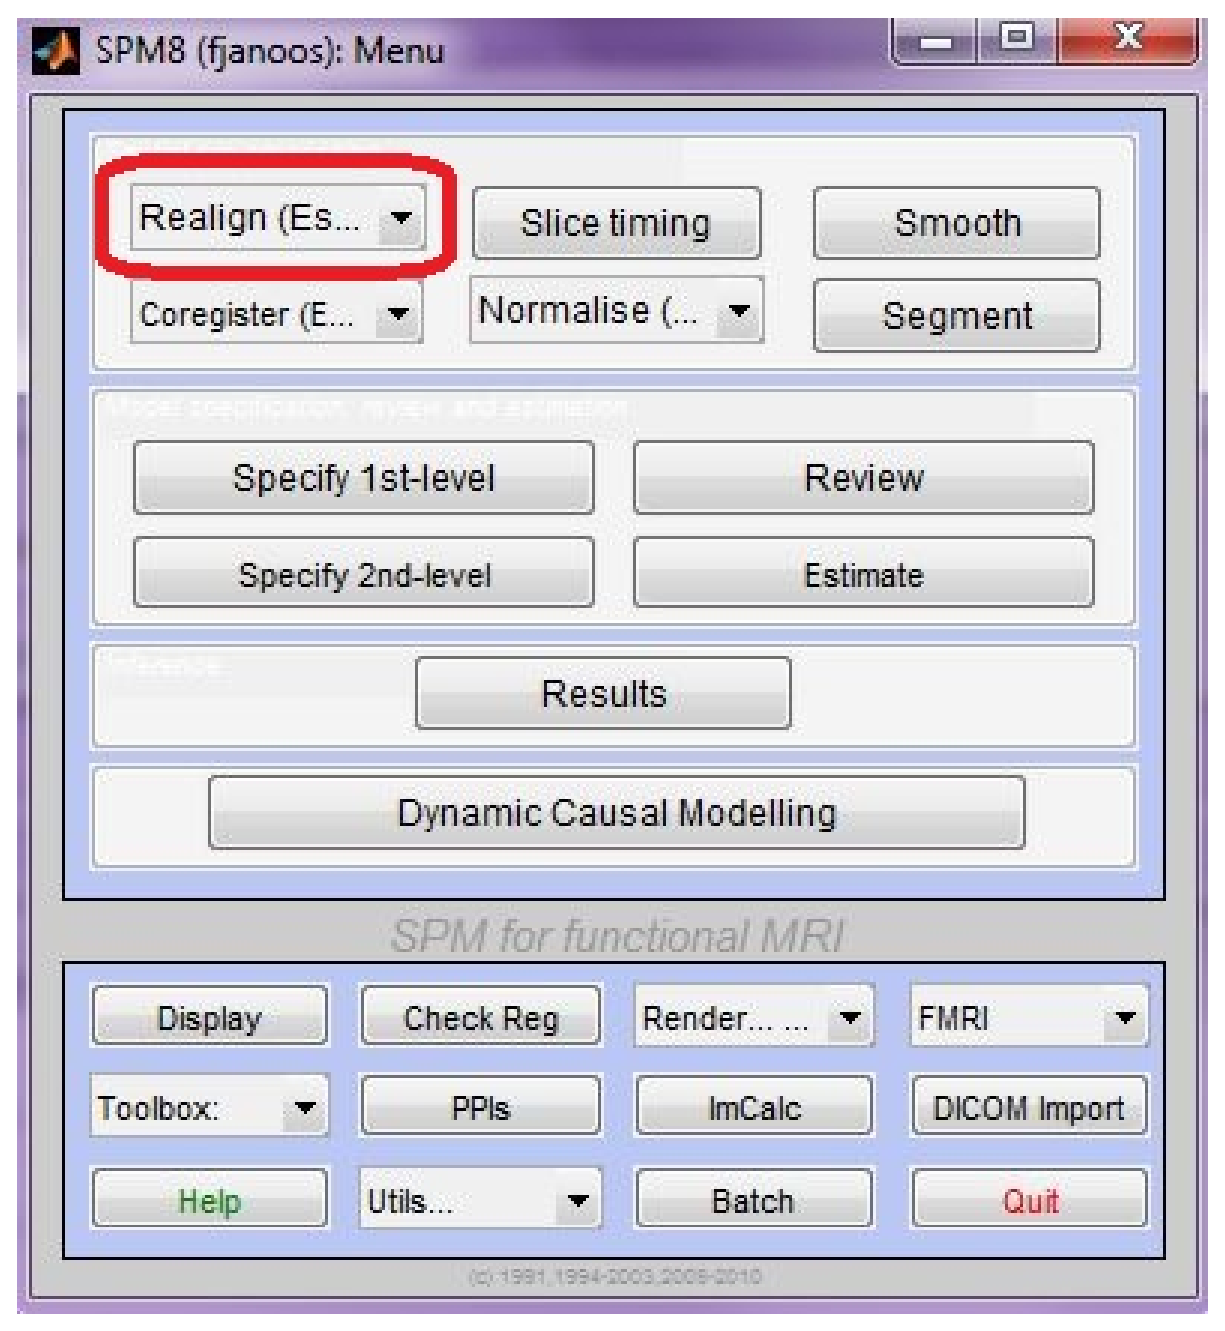
\includegraphics[width=.37\linewidth]{figures/spm-est_res}
    \caption[Estimate and Reslice Option of SPM8.]
    {Estimate and Reslice Option of SPM8.\label{fig:spm-est_res}}
    \end{center}
\end{figure}
Use the slice timing and motion correction modules from SPM5. For
motion correction, apply the \verb"Estimate and Reslice" operations
(\cf~\Fig{fig:spm-est_res}).

In order to remove residual motion artifacts from the time-series
data (described in the next section), build a design matrix
consisting only of the motion parameters estimated by SPM
(\verb"rp_*.txt"), and save it as an \verb"SPM.mat" file\footnote{By
selecting the file in the { Multiple Regressors} field of the SPM {
Specify 1st-level} GUI. Do not include regressors for any
experimental conditions}.

For details, refer to the SPM Manual\cite{TheFILMethodsGroup2011}.

\section{Motion Artifact Removal with GIFT}

\begin{figure}
    \begin{center}
   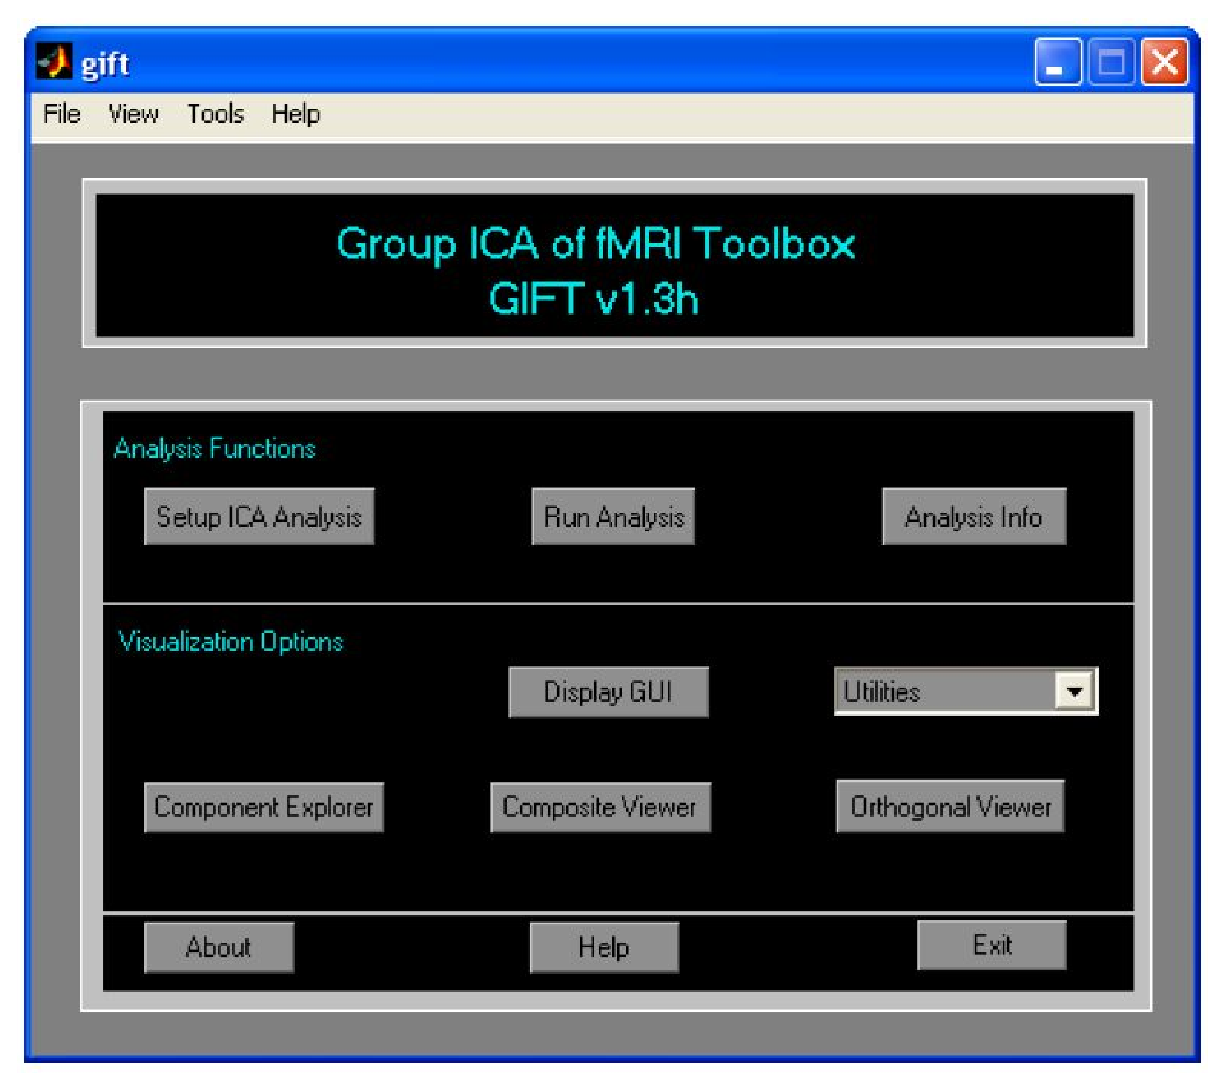
\includegraphics[width=.5\linewidth]{figures/gift}
    \caption[Group ICA for fMRI Toolbox (GIFT)]
    {Group ICA for fMRI Toolbox (GIFT).
     \label{fig:gift}}
    \end{center}
\end{figure}
The motion correction operation itself tends to introduce strong
artifacts \citet{Grootoonk2000}. These artifacts are removed using
ICA analysis with GIFT (\cf~\Fig{fig:gift}). For this, first start
up GIFT and configure it for analysis of an individual
session(\cf~\Fig{fig:gift-setup}). Set the number of ICA to that
automatically estimated by GIFT. Set ICA Algorithm to Infomax and
Group ICA Analysis to Regular. Use the setup defaults for all other
settings.

\begin{figure}
    \begin{center}
   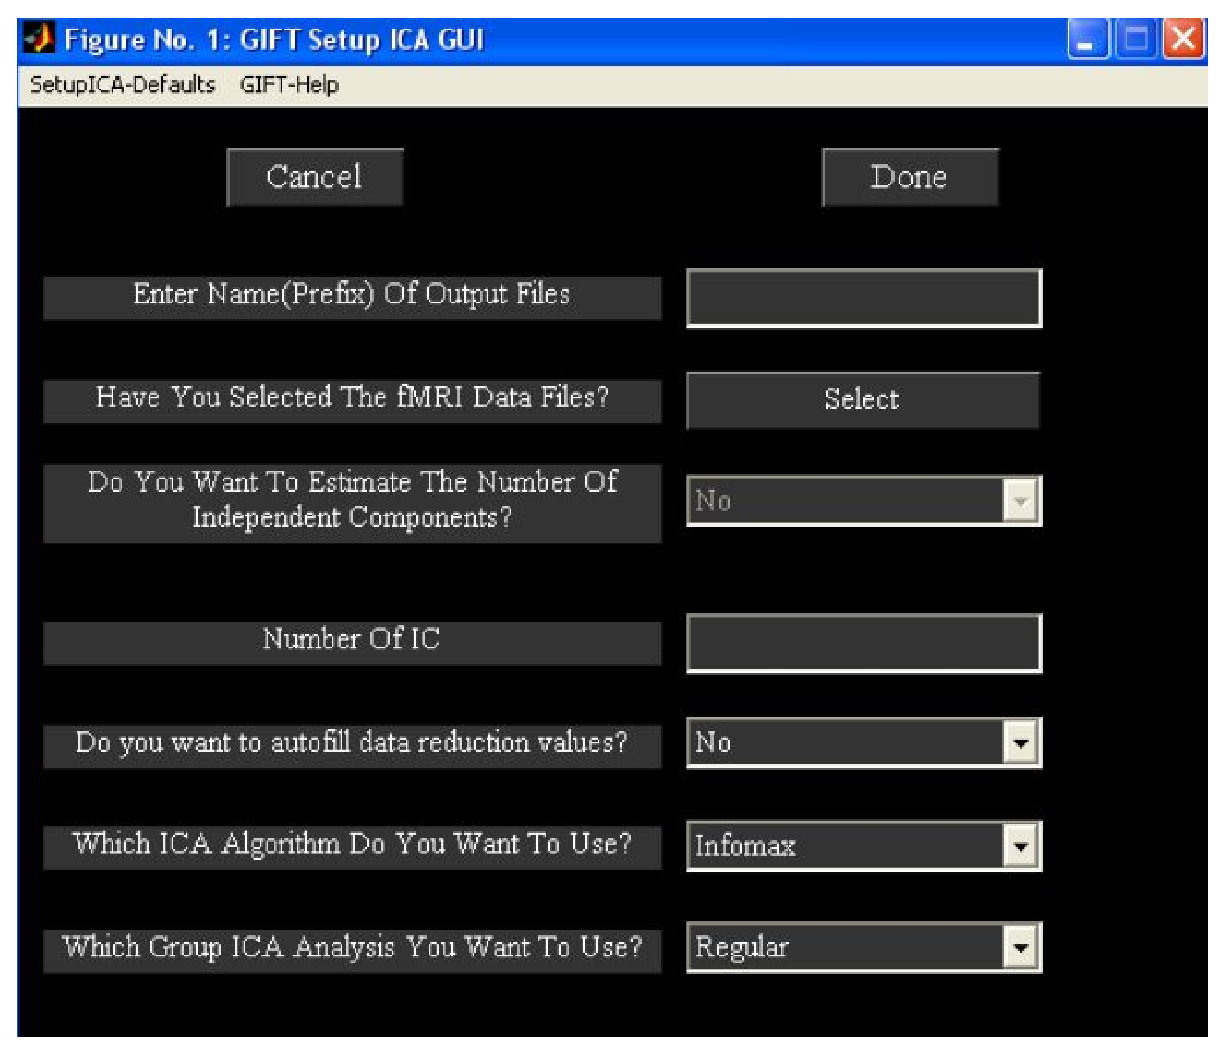
\includegraphics[width=.5\linewidth]{figures/gift-ica-setup}
    \caption[Configuring a GIFT analysis session.]
    {Configuring a GIFT analysis session.
     \label{fig:gift-setup}}
    \end{center}
\end{figure}

After configuring the GIFT analysis, run all the analysis steps
\begin{figure}
    \begin{center}
   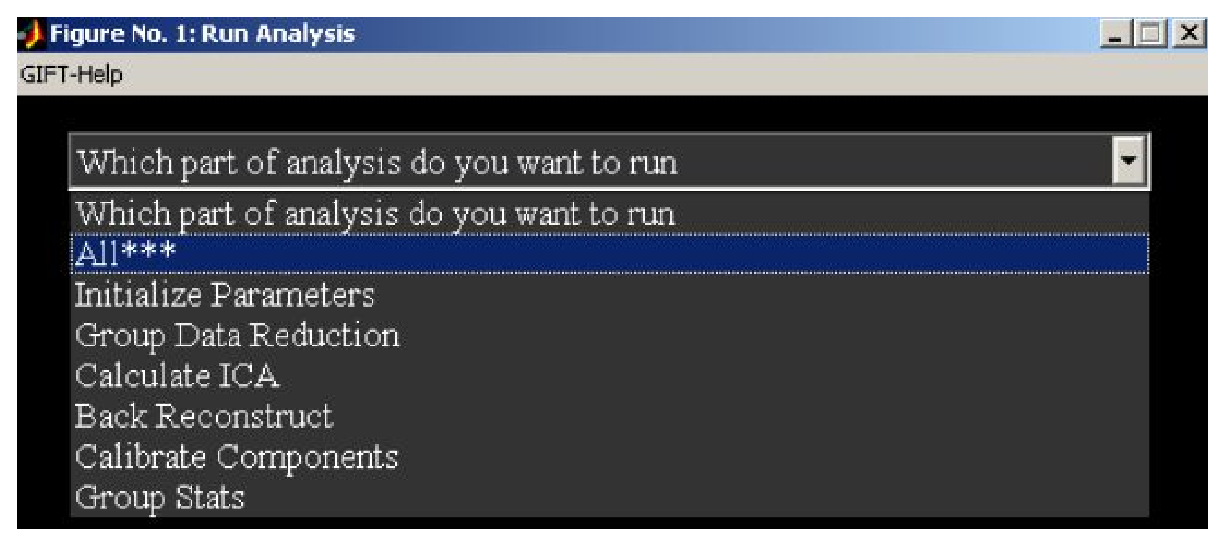
\includegraphics[width=.5\linewidth]{figures/gift-run}
    \caption[Group ICA for fMRI Toolbox (GIFT).]{Group ICA for fMRI Toolbox (GIFT).
     \label{fig:gift-setup}}
    \end{center}
\end{figure}

After the analysis is complete, open the \verb"Component Explorer"
and select the generated parameter file. Now, identify components of
artifactual origin using one of two methods:

\begin{enumerate}[a]
  \item Manual inspection of components for high concentration of
  intensity close to vessicles, tissue interfaces and image
  boundaries.
  \item Sorting component through multiple regression against motion
  parameters estimated in \Sec{sec:slc-tim}. This can be
  achieved the \verb"Sort Components" feature of the visualization
  GUI and providing the design matrix of the SPM.mat file containing
  regressors built from the motion parameters (\cf~\Fig{fig:gift-regress}).
\end{enumerate}

\begin{figure}
    \begin{center}
   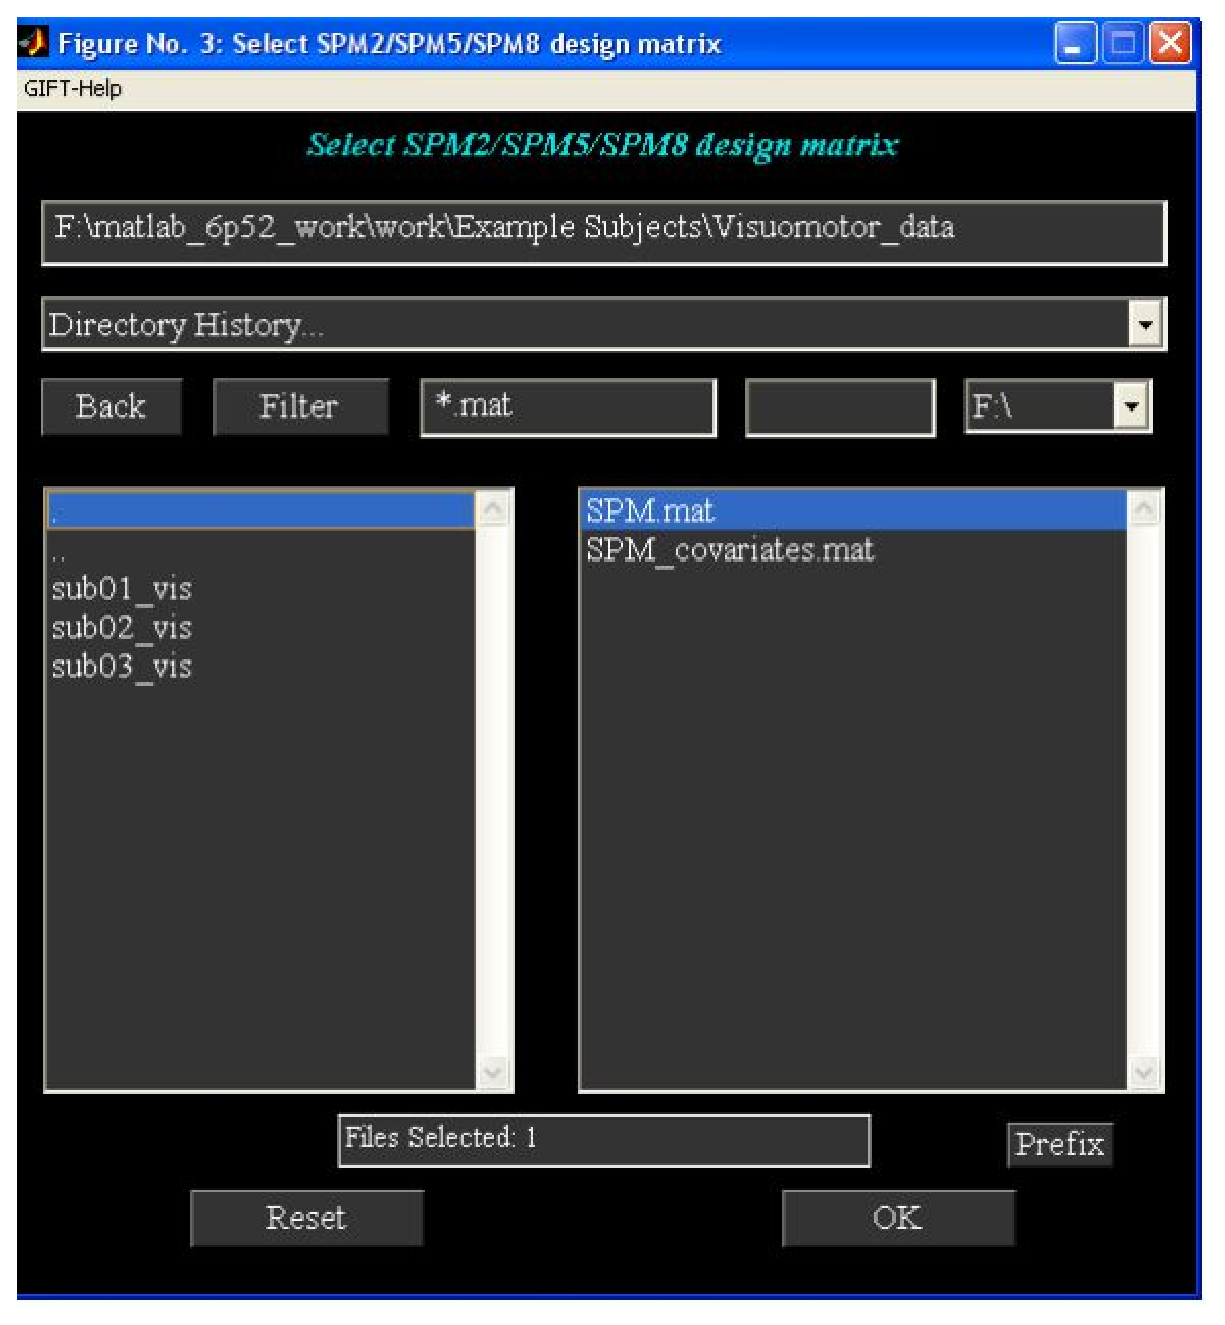
\includegraphics[width=.37\linewidth]{figures/gift-regress}
    \caption{Sorting components through regression in GIFT.
     \label{fig:gift-regress}}
    \end{center}
\end{figure}

After the artifactual components have been identified, they can be
effectively removed from the time-series data through the \verb"Back Reconstruction"
facility available in GIFT.

Please refer to the GIFT manual for more details.

\section{De-noising}

The preferred method of removing random $1/f$--type noise present in the fMRI time-course data
is a wavelet based algorithm \cite{Alexander2000}, that used a Wiener-type shrinkage for thresholding
noise coefficient.

For this, the steps are as follows, in MATLAB\footnote{Make sure to use a copy of the original data, as this
routine will overwrite the volumes in the vi structure.}:
\begin{verbatim}
    \% load the fmri dataset
    vi = spm_vol( epi_series_copy_fnames );
    preprocWaveletDenoise(vi, 'daubechies', 'wiener');
\end{verbatim}

The options for
\begin{verbatim}
preprocWaveletDenoise( epi\_vol\_info\_struct,
 wavelet\_type, shrinkage\_type )
\end{verbatim}
are:
\begin{itemize}
  \item \verb"epi\_vol\_info\_struct" - the array of \verb"spm\_vol" structures of the EPI time-series. Note that the
  files pointed to by these structures are used both as input and output of the denoising routine.
  \item \verb"wavelet\_type" - Valid choices are \verb"daubechies", \verb"haar", or \verb"cdf97".
  \item \verb"shrinkage\_type" - Valid options are \verb"hard", \verb"soft", \verb"sure", \verb"wiener".
\end{itemize}

Next, the time--series data are high-pass filtered ($0.5$Hz) to remove artifacts due
to breathing, blood pressure changes and scanner drift. Further polynomial trends are also eliminated through
polynomial regression\footnote{The method uses a complex analytic representation of the signal and of
a Legendre polynomial basis for regression.}.

For this, use the same \verb"spm\_vol" structure array obtained from above as input to
\begin{verbatim}
preprocDetrend( epi\_vol\_info\_struct,
freq\_cutoff, poly\_order )
\end{verbatim}
are:
\begin{itemize}
  \item \verb"epi\_vol_info_struct" - the array of \verb"spm\_vol" structures of the EPI time-series. Note that the
  files pointed to by these structures are used both as input and output of the denoising routine.
  \item \verb"freq\_cutoff" - The upper frequency for truncation.
  \item \verb"poly\_order" - The highest order of the polynomial for detrending.
\end{itemize}
%
%TODO: The frequency filtering and polynomial detrending can also be done in the wavelet basis. Need to integrate them into
%the denoising step.
